% !TeX program = xelatex
%
% Лекция-сопровождение к лабораторной работе № 1 «Классификация текстов».
%
% Сборка:  xelatex mlg_lab1_classification.tex   (дважды)
% Оформление и макросы — в mlg_preamble.tex, общем для всех лекций курса.
% Все числа посчитаны на учебном корпусе курса и закреплены тестами
% репозитория gd_learn; придуманных чисел на слайдах нет.
%
\documentclass[aspectratio=169,12pt]{beamer}

% Общая преамбула лекций курса. Подключается после \documentclass:
%
%     \documentclass[aspectratio=169,12pt]{beamer}
%     % Общая преамбула лекций курса. Подключается после \documentclass:
%
%     \documentclass[aspectratio=169,12pt]{beamer}
%     % Общая преамбула лекций курса. Подключается после \documentclass:
%
%     \documentclass[aspectratio=169,12pt]{beamer}
%     \input{mlg_preamble}
%
% Здесь только оформление и макросы — ни \title, ни текста слайдов, чтобы
% пять презентаций курса выглядели одинаково и правились в одном месте.
%
\usepackage{fontspec}
\usepackage{polyglossia}
\setmainlanguage{russian}
\setotherlanguage{english}
\setmainfont{Calibri}
\setsansfont{Calibri}
\setmonofont{Consolas}[Scale=0.92]

\usepackage{graphicx}
\usepackage{booktabs}
\usepackage{array}

% ---------------------------------------------------------------- оформление
\definecolor{ink}{HTML}{1B2433}
\definecolor{navy}{HTML}{2B4C6F}
\definecolor{brick}{HTML}{B03A2B}
\definecolor{moss}{HTML}{3E7D5A}
\definecolor{plum}{HTML}{6B5B95}
\definecolor{ash}{HTML}{8B9299}
\definecolor{paper}{HTML}{ECEFF3}

\usetheme{default}
\usecolortheme{default}
\setbeamercolor{structure}{fg=navy}
\setbeamercolor{frametitle}{fg=navy}
\setbeamercolor{normal text}{fg=ink}
\setbeamercolor{itemize item}{fg=navy}
\setbeamercolor{itemize subitem}{fg=ash}
\setbeamerfont{frametitle}{size=\Large,series=\bfseries}
\setbeamerfont{framesubtitle}{size=\small,series=\mdseries}
\setbeamercolor{framesubtitle}{fg=ash}
\setbeamertemplate{navigation symbols}{}
\setbeamertemplate{itemize item}{\raisebox{0.15ex}{\tiny$\bullet$}}
\setbeamertemplate{itemize subitem}{\raisebox{0.15ex}{\tiny--}}
\setbeamersize{text margin left=1.1cm, text margin right=1.1cm}

\setbeamertemplate{footline}{%
  \hbox{\begin{beamercolorbox}[wd=\paperwidth,ht=2.6ex,dp=1.4ex,leftskip=1.1cm,%
        rightskip=1.1cm]{}%
    {\color{ash}\scriptsize Основы машинного обучения \quad·\quad
     Цифровая лингвистика и локализация}\hfill
    {\color{ash}\scriptsize\insertframenumber}%
  \end{beamercolorbox}}}

% Врезка: связь слайда с лабораторной или с работой переводчика.
% Ширина считается точно: colorbox добавляет \fboxsep с каждой стороны,
% поэтому parbox должен быть на 2\fboxsep уже текстового поля — иначе
% на каждом слайде вылезает overfull hbox.
\newcommand{\врезка}[1]{%
  \par\vspace{0.5ex}\noindent
  \colorbox{paper}{%
    \parbox{\dimexpr\textwidth-2\fboxsep\relax}{%
      \vspace{0.7ex}\small #1\vspace{0.7ex}}}\par}

% Колонка таблицы заданной доли ширины, без растягивания пробелов.
% Объявлять её нужно здесь: внутри frame beamer пересканирует тело кадра,
% и #1 в определении вызывает «Illegal parameter number».
\newcolumntype{Л}[1]{>{\raggedright\arraybackslash}p{#1\textwidth}}

% Ссылка на интерактивную страницу к слайду. Playground'ы считают те же
% числа на том же корпусе, что и лабораторные, поэтому на них можно
% ссылаться прямо с лекции, не оговаривая расхождений.
\hypersetup{colorlinks=true,urlcolor=moss,linkcolor=moss}
\newcommand{\playground}[3]{%
  \par\vspace{0.4ex}%
  {\footnotesize\color{ash}$\rightarrow$~\href{#1}{\bfseries #2} — #3\par}}

\newcommand{\кейс}[1]{{\color{brick}\small\textbf{#1}}}
\newcommand{\числ}[1]{{\color{navy}\bfseries #1}}

%
% Здесь только оформление и макросы — ни \title, ни текста слайдов, чтобы
% пять презентаций курса выглядели одинаково и правились в одном месте.
%
\usepackage{fontspec}
\usepackage{polyglossia}
\setmainlanguage{russian}
\setotherlanguage{english}
\setmainfont{Calibri}
\setsansfont{Calibri}
\setmonofont{Consolas}[Scale=0.92]

\usepackage{graphicx}
\usepackage{booktabs}
\usepackage{array}

% ---------------------------------------------------------------- оформление
\definecolor{ink}{HTML}{1B2433}
\definecolor{navy}{HTML}{2B4C6F}
\definecolor{brick}{HTML}{B03A2B}
\definecolor{moss}{HTML}{3E7D5A}
\definecolor{plum}{HTML}{6B5B95}
\definecolor{ash}{HTML}{8B9299}
\definecolor{paper}{HTML}{ECEFF3}

\usetheme{default}
\usecolortheme{default}
\setbeamercolor{structure}{fg=navy}
\setbeamercolor{frametitle}{fg=navy}
\setbeamercolor{normal text}{fg=ink}
\setbeamercolor{itemize item}{fg=navy}
\setbeamercolor{itemize subitem}{fg=ash}
\setbeamerfont{frametitle}{size=\Large,series=\bfseries}
\setbeamerfont{framesubtitle}{size=\small,series=\mdseries}
\setbeamercolor{framesubtitle}{fg=ash}
\setbeamertemplate{navigation symbols}{}
\setbeamertemplate{itemize item}{\raisebox{0.15ex}{\tiny$\bullet$}}
\setbeamertemplate{itemize subitem}{\raisebox{0.15ex}{\tiny--}}
\setbeamersize{text margin left=1.1cm, text margin right=1.1cm}

\setbeamertemplate{footline}{%
  \hbox{\begin{beamercolorbox}[wd=\paperwidth,ht=2.6ex,dp=1.4ex,leftskip=1.1cm,%
        rightskip=1.1cm]{}%
    {\color{ash}\scriptsize Основы машинного обучения \quad·\quad
     Цифровая лингвистика и локализация}\hfill
    {\color{ash}\scriptsize\insertframenumber}%
  \end{beamercolorbox}}}

% Врезка: связь слайда с лабораторной или с работой переводчика.
% Ширина считается точно: colorbox добавляет \fboxsep с каждой стороны,
% поэтому parbox должен быть на 2\fboxsep уже текстового поля — иначе
% на каждом слайде вылезает overfull hbox.
\newcommand{\врезка}[1]{%
  \par\vspace{0.5ex}\noindent
  \colorbox{paper}{%
    \parbox{\dimexpr\textwidth-2\fboxsep\relax}{%
      \vspace{0.7ex}\small #1\vspace{0.7ex}}}\par}

% Колонка таблицы заданной доли ширины, без растягивания пробелов.
% Объявлять её нужно здесь: внутри frame beamer пересканирует тело кадра,
% и #1 в определении вызывает «Illegal parameter number».
\newcolumntype{Л}[1]{>{\raggedright\arraybackslash}p{#1\textwidth}}

% Ссылка на интерактивную страницу к слайду. Playground'ы считают те же
% числа на том же корпусе, что и лабораторные, поэтому на них можно
% ссылаться прямо с лекции, не оговаривая расхождений.
\hypersetup{colorlinks=true,urlcolor=moss,linkcolor=moss}
\newcommand{\playground}[3]{%
  \par\vspace{0.4ex}%
  {\footnotesize\color{ash}$\rightarrow$~\href{#1}{\bfseries #2} — #3\par}}

\newcommand{\кейс}[1]{{\color{brick}\small\textbf{#1}}}
\newcommand{\числ}[1]{{\color{navy}\bfseries #1}}

%
% Здесь только оформление и макросы — ни \title, ни текста слайдов, чтобы
% пять презентаций курса выглядели одинаково и правились в одном месте.
%
\usepackage{fontspec}
\usepackage{polyglossia}
\setmainlanguage{russian}
\setotherlanguage{english}
\setmainfont{Calibri}
\setsansfont{Calibri}
\setmonofont{Consolas}[Scale=0.92]

\usepackage{graphicx}
\usepackage{booktabs}
\usepackage{array}

% ---------------------------------------------------------------- оформление
\definecolor{ink}{HTML}{1B2433}
\definecolor{navy}{HTML}{2B4C6F}
\definecolor{brick}{HTML}{B03A2B}
\definecolor{moss}{HTML}{3E7D5A}
\definecolor{plum}{HTML}{6B5B95}
\definecolor{ash}{HTML}{8B9299}
\definecolor{paper}{HTML}{ECEFF3}

\usetheme{default}
\usecolortheme{default}
\setbeamercolor{structure}{fg=navy}
\setbeamercolor{frametitle}{fg=navy}
\setbeamercolor{normal text}{fg=ink}
\setbeamercolor{itemize item}{fg=navy}
\setbeamercolor{itemize subitem}{fg=ash}
\setbeamerfont{frametitle}{size=\Large,series=\bfseries}
\setbeamerfont{framesubtitle}{size=\small,series=\mdseries}
\setbeamercolor{framesubtitle}{fg=ash}
\setbeamertemplate{navigation symbols}{}
\setbeamertemplate{itemize item}{\raisebox{0.15ex}{\tiny$\bullet$}}
\setbeamertemplate{itemize subitem}{\raisebox{0.15ex}{\tiny--}}
\setbeamersize{text margin left=1.1cm, text margin right=1.1cm}

\setbeamertemplate{footline}{%
  \hbox{\begin{beamercolorbox}[wd=\paperwidth,ht=2.6ex,dp=1.4ex,leftskip=1.1cm,%
        rightskip=1.1cm]{}%
    {\color{ash}\scriptsize Основы машинного обучения \quad·\quad
     Цифровая лингвистика и локализация}\hfill
    {\color{ash}\scriptsize\insertframenumber}%
  \end{beamercolorbox}}}

% Врезка: связь слайда с лабораторной или с работой переводчика.
% Ширина считается точно: colorbox добавляет \fboxsep с каждой стороны,
% поэтому parbox должен быть на 2\fboxsep уже текстового поля — иначе
% на каждом слайде вылезает overfull hbox.
\newcommand{\врезка}[1]{%
  \par\vspace{0.5ex}\noindent
  \colorbox{paper}{%
    \parbox{\dimexpr\textwidth-2\fboxsep\relax}{%
      \vspace{0.7ex}\small #1\vspace{0.7ex}}}\par}

% Колонка таблицы заданной доли ширины, без растягивания пробелов.
% Объявлять её нужно здесь: внутри frame beamer пересканирует тело кадра,
% и #1 в определении вызывает «Illegal parameter number».
\newcolumntype{Л}[1]{>{\raggedright\arraybackslash}p{#1\textwidth}}

% Ссылка на интерактивную страницу к слайду. Playground'ы считают те же
% числа на том же корпусе, что и лабораторные, поэтому на них можно
% ссылаться прямо с лекции, не оговаривая расхождений.
\hypersetup{colorlinks=true,urlcolor=moss,linkcolor=moss}
\newcommand{\playground}[3]{%
  \par\vspace{0.4ex}%
  {\footnotesize\color{ash}$\rightarrow$~\href{#1}{\bfseries #2} — #3\par}}

\newcommand{\кейс}[1]{{\color{brick}\small\textbf{#1}}}
\newcommand{\числ}[1]{{\color{navy}\bfseries #1}}


\title{Лабораторная работа № 1}
\subtitle{Классификация текстов}
\date{}
\author{}

\begin{document}

% =====================================================================
\begin{frame}[plain]
  \vspace{1.2cm}
  {\color{brick}\small\bfseries ЛАБОРАТОРНАЯ РАБОТА № 1}

  \vspace{0.7cm}
  {\color{navy}\fontsize{30}{34}\selectfont\bfseries Классификация текстов\par}

  \vspace{0.5cm}
  {\color{ink}\large Как лингвистическое решение превращается в число\par}

  \vspace{1.0cm}
  {\color{ash} Корпус: 160 сегментов локализации, четыре типа контента.
   Все числа на слайдах получены на нём и проверяются автоматически
   при каждом изменении кода.\par}
\end{frame}

% =====================================================================
\begin{frame}{Что делаем в этой работе}
  Задача: по тексту сегмента определить, к какому типу контента он относится.
  Это настоящая задача локализации — от типа зависит, кому сегмент отдавать
  и по какой ставке.

  \vspace{0.8em}
  \begin{columns}[T,onlytextwidth]
    \column{0.47\textwidth}
      {\color{navy}\bfseries Техническая часть}\\[0.4em]
      {\small Четыре шага scikit-learn, базовое решение, векторизация,
      матрица ошибок. Это каркас, он одинаков для любой задачи
      классификации.}
    \column{0.47\textwidth}
      {\color{brick}\bfseries Главная часть}\\[0.4em]
      {\small Как предобработка текста влияет на качество — и почему
      именно так. Ответ на «почему» должен быть лингвистическим, а не
      «так вышло».}
  \end{columns}

  \vspace{1.0em}
  \врезка{\textbf{Что оценивается.} Не точность вашей модели. Объяснение,
  почему одна настройка признаков обыграла другую. Модель обучает
  библиотека, объясняет лингвист.}
\end{frame}

% =====================================================================
\begin{frame}{Данные}
  \begin{columns}[T,onlytextwidth]
    \column{0.54\textwidth}
      \vspace{0.1cm}
      {\small
      \begin{tabular}{@{}l@{\hspace{1em}}l@{}}
        \toprule
        тип & что это \\
        \midrule
        \texttt{интерфейс}    & кнопки, подсказки, ошибки \\
        \texttt{документация} & руководства, справка \\
        \texttt{маркетинг}    & рекламные тексты \\
        \texttt{юридический}  & договоры, политики \\
        \bottomrule
      \end{tabular}}

      \vspace{0.9em}
      {\small По \числ{40} сегментов каждого типа — корпус сбалансирован
      намеренно.}
    \column{0.42\textwidth}
      {\small
      Столбцы корпуса:\par
      \vspace{0.5em}
      \texttt{en} — исходный текст\par
      \texttt{ru\_ref} — эталонный перевод\par
      \texttt{ru\_mt} — машинный перевод\par
      \vspace{0.8em}
      В этой работе используется только \texttt{ru\_ref}.
      \texttt{ru\_mt} понадобится в работе № 3.}
  \end{columns}

  \vspace{1.0em}
  \врезка{\textbf{160 сегментов — это мало.} Настолько мало, что одна
  случайная разбивка на обучение и контроль ничего не докажет. Поэтому
  везде дальше — пятикратная кросс-валидация, и рядом с точностью всегда
  стоит разброс между долями.}
\end{frame}

% =====================================================================
\begin{frame}{Базовое решение: с чем сравнивать}
  Прежде чем радоваться точности, нужно знать, сколько даёт
  \emph{бессмысленная} модель. Иначе «точность 0,5» ни о чём не говорит.

  \vspace{0.9em}
  \begin{columns}[T,onlytextwidth]
    \column{0.47\textwidth}
      {\color{navy}\bfseries Наивнее некуда}\\[0.4em]
      {\small Всегда отвечать самым частым классом. На сбалансированном
      корпусе из четырёх типов это ровно одна четверть.\par
      \vspace{0.7em}
      \числ{0{,}250} — вот отметка, выше которой начинается смысл.}
    \column{0.47\textwidth}
      {\color{brick}\bfseries Зачем это нужно в проекте}\\[0.4em]
      {\small Заказчик спросит «модель хорошая?». Правильный ответ —
      «лучше базового решения на столько-то», а не абсолютное число.\par
      \vspace{0.7em}
      На несбалансированных данных baseline бывает 0,9 — и тогда
      «точность 0,88» означает, что модель хуже, чем ничего.}
  \end{columns}
\end{frame}

% =====================================================================
\begin{frame}{Текст → числа}
  \begin{columns}[T,onlytextwidth]
    \column{0.44\textwidth}
      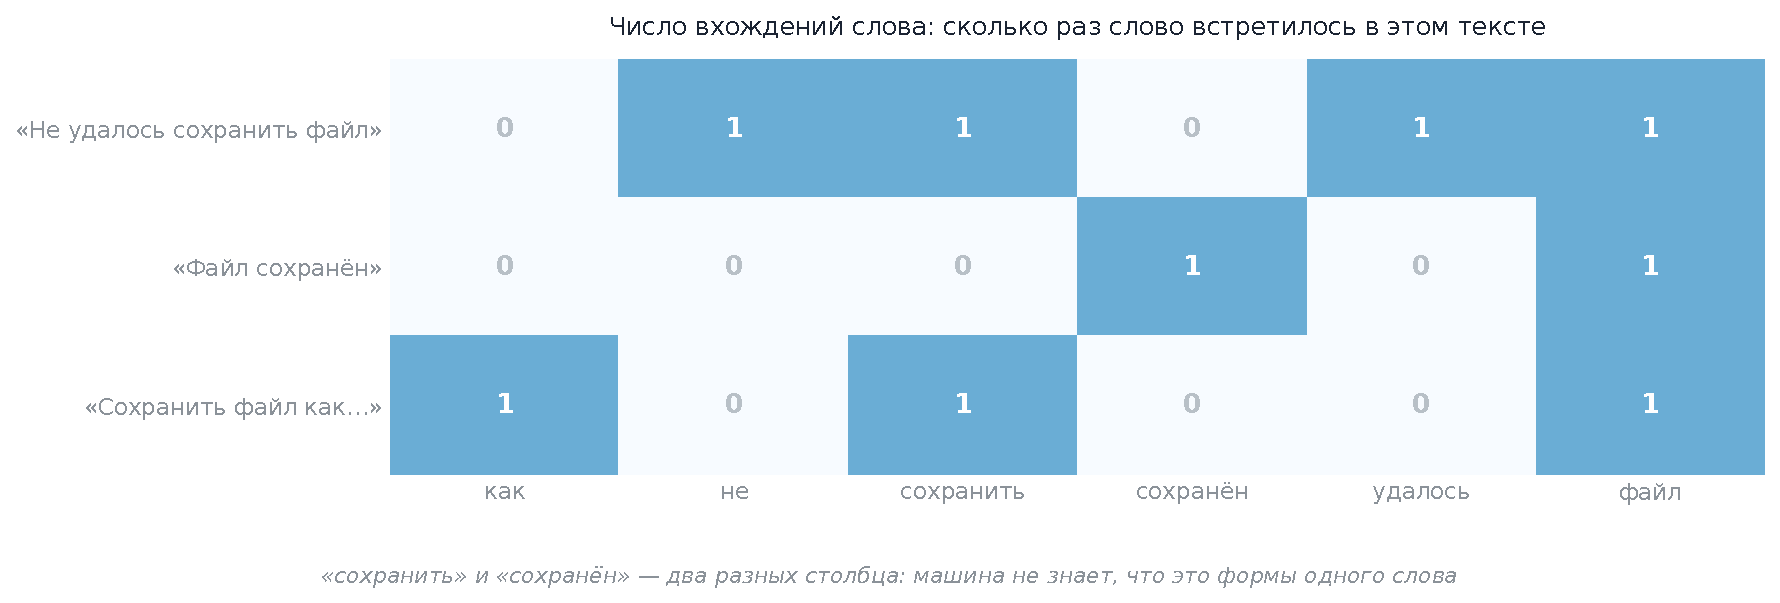
\includegraphics[width=\textwidth]{fig/bagofwords.pdf}
    \column{0.52\textwidth}
      \vspace{0.1cm}
      {\small
      Модель не видит текста. Она видит таблицу чисел, и всё, что вы
      знаете о языке, попадает в неё ровно одним способом — через то,
      \textbf{как вы построили эту таблицу}.\par
      \vspace{0.8em}
      {\color{navy}\bfseries Мешок слов:} сколько раз встретилось слово.
      Порядок слов теряется полностью.\par
      \vspace{0.6em}
      {\color{navy}\bfseries TF-IDF:} то же, но частые во всём корпусе
      слова весят меньше. «Настройки» в корпусе локализации — почти
      служебное слово.}
  \end{columns}

  \playground{https://konkin-nikita.ru/gd_learn/vec/}{векторизация текста}%
  {признаки переключаются мышью, число столбцов видно сразу.}
\end{frame}

% =====================================================================
\begin{frame}{Первый результат}
  \begin{columns}[T,onlytextwidth]
    \column{0.47\textwidth}
      {\small
      TF-IDF по словам, настройки по умолчанию, наивный Байес
      (раздел 7):\par
      \vspace{0.6em}
      {\color{navy}\fontsize{26}{28}\selectfont\bfseries 0,444\par}
      \vspace{0.6em}
      Базовое решение — 0,250. Почти вдвое лучше бессмыслицы, и это всё,
      что пока можно сказать.\par
      \vspace{0.7em}
      Признаков: \числ{679} — столько разных слов в 160 сегментах.}
    \column{0.47\textwidth}
      \врезка{\textbf{Разброс между долями — 0,085.} На одной пятой
      корпуса модель даёт 0,31, на другой 0,56. Любое сравнение двух
      настроек, различающихся на 0,02, — это сравнение шума с
      шумом.\par
      \vspace{0.5em}
      В отчёте разброс приводить обязательно.}
  \end{columns}
\end{frame}

% =====================================================================
\begin{frame}{Какие ошибки делает модель}
  \begin{columns}[T,onlytextwidth]
    \column{0.46\textwidth}
      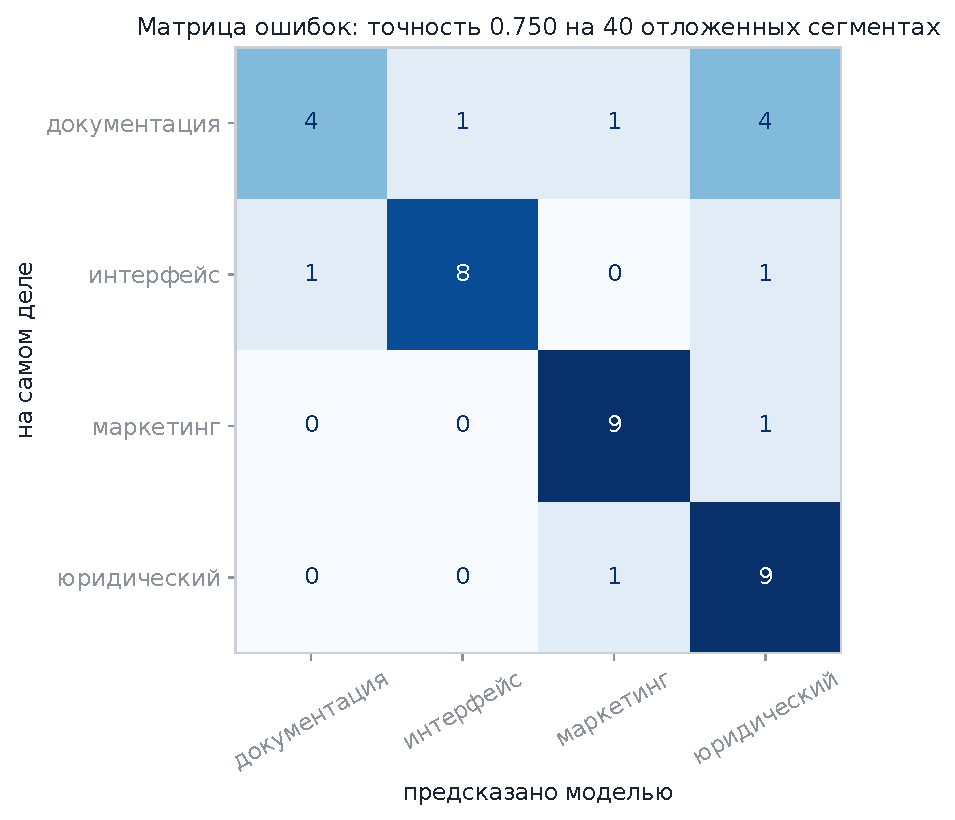
\includegraphics[width=\textwidth]{fig/confusion.pdf}
    \column{0.50\textwidth}
      \vspace{0.1cm}
      {\small
      Матрица ошибок отвечает не на вопрос «сколько ошибок», а на вопрос
      \emph{какие}: какой класс с каким смешивается.\par
      \vspace{0.7em}
      {\color{brick}\bfseries Читается по-лингвистически:} путаются
      документация, маркетинг и юридический текст — все трое состоят из
      полных предложений с подлежащим и сказуемым.\par
      \vspace{0.6em}
      Интерфейс не путается почти ни с чем: короткие безглагольные
      строки, часто без финальной точки, ни на что больше не похожи.}
  \end{columns}

  \playground{https://konkin-nikita.ru/gd_learn/vec/}{векторизация текста}%
  {та же матрица, но признаки переключаются на ходу.}
\end{frame}

% =====================================================================
\begin{frame}{Лингвистическая предобработка: стемминг}
  Русский язык флективный: «настройка», «настройки», «настройкам»,
  «настройками» — для мешка слов это четыре разных редких признака.

  \vspace{0.2em}
  \begin{columns}[T,onlytextwidth]
    \column{0.47\textwidth}
      {\color{moss}\bfseries Что делает стемминг}\\[0.4em]
      {\small Отрезает окончание, сводя все формы к одной основе. Четыре
      редких признака становятся одним частым.\par
      \vspace{0.4em}
      Точность: \числ{0{,}444} $\rightarrow$ \числ{0{,}538}.\par
      Признаков: 679 $\rightarrow$ 555.}
    \column{0.47\textwidth}
      {\color{brick}\bfseries Чего он не делает}\\[0.4em]
      {\small Стеммер режет по правилам, а не по словарю: он одинаково
      спокойно отрежет то, что окончанием не является.\par
      \vspace{0.4em}
      Это не лемматизация. Основы, которые он выдаёт, могут не быть
      словами русского языка — и это нормально, модели слова не нужны.}
  \end{columns}

  \vspace{0.2em}
  \врезка{\textbf{+0,094 при разбросе до 0,135:} планки перекрываются, и по
  одной таблице стемминг лучшим не назвать.}
\end{frame}

% =====================================================================
\begin{frame}{Главный результат работы}
  \begin{columns}[T,onlytextwidth]
    \column{0.47\textwidth}
      {\small
      Признаки не по словам, а по \textbf{буквосочетаниям внутри слов} —
      символьные n-граммы. На том же Байесе:\par
      \vspace{0.5em}
      {\color{navy}\fontsize{26}{28}\selectfont\bfseries 0,612–0,631\par}
      \vspace{0.5em}
      Стемминг — 0,538, слова — 0,444.\par
      \vspace{0.5em}
      «настройк», «астрой», «строй» — модель получает основу, не зная о
      существовании основ.}
    \column{0.47\textwidth}
      {\color{brick}\bfseries Почему это работает на русском}\\[0.4em]
      {\small Символьные n-граммы решают морфологическую проблему
      \emph{мимо} морфологии. Совпадающие куски слов у разных словоформ
      общие — этого достаточно.\par
      \vspace{0.6em}
      Побочно ловится и то, чего стеммер не видит: опечатки, латиница
      внутри русского текста, плейсхолдеры.}
  \end{columns}

  \vspace{0.7em}
  \врезка{\textbf{Цена:} \числ{5418}–\числ{7821} признаков вместо 679. На 160
  сегментах это мгновенно, на миллионе — уже нет.}
\end{frame}

% =====================================================================
\begin{frame}{Все настройки рядом}
  \vspace{-0.2em}
  {\small
  \begin{tabular}{@{}Л{0.30}rrr@{}}
    \toprule
    конфигурация & точность & разброс & признаков \\
    \midrule
    базовое решение          & 0,250 & --- & --- \\
    TF-IDF по умолчанию      & 0,444 & 0,085 & 679 \\
    без нижнего регистра     & 0,419 & 0,064 & 705 \\
    со стоп-словами          & 0,419 & 0,090 & 637 \\
    слова + биграммы         & 0,456 & 0,076 & 1381 \\
    \texttt{min\_df=2}       & 0,381 & 0,061 & 99 \\
    стемминг                 & 0,538 & 0,135 & 555 \\
    \textbf{символьные 3–5}  & \числ{0{,}631} & 0,098 & 7821 \\
    символьные 2–4           & 0,612 & 0,102 & 5418 \\
    \bottomrule
  \end{tabular}}

  \vspace{0.6em}
  {\small Наивный Байес, пятикратная кросс-валидация — таблица раздела 8.
  Отказ от нижнего регистра и стоп-слова \emph{ухудшают} результат,
  \texttt{min\_df=2} выбрасывает редкие слова — и с ними почти всю
  различающую информацию. 3–5 и 2–4 расходятся на 0,019 при разбросе
  0,1: разница не установлена.}
\end{frame}

% =====================================================================
\begin{frame}{Модель тоже важна — но меньше}
  Раздел 9: лучшие признаки (символьные 2–4) оставляем, меняем классификатор.

  \vspace{0.5em}
  {\small
  \begin{tabular}{@{}Л{0.34}rr@{}}
    \toprule
    модель & точность & разброс \\
    \midrule
    наивный Байес            & 0,612 & 0,102 \\
    логистическая регрессия  & \числ{0{,}744} & 0,100 \\
    ближайшие соседи, $k=5$  & 0,550 & 0,064 \\
    \bottomrule
  \end{tabular}}

  \vspace{0.6em}
  {\small Модели расходятся на \числ{0{,}19}; предобработка на одном Байесе —
  на \числ{0{,}25}. Признаки чуть сильнее, но это величины одного порядка.}

  \врезка{\textbf{Признаки и модель выбирают вместе.} С Байесом чуть лучше
  смотрелись n-граммы 3–5, с логистической регрессией выигрывают 2–4:
  0,744 против 0,713.}

  \playground{https://konkin-nikita.ru/gd_learn/vec/}{векторизация текста}%
  {модель и длина n-грамм — два переключателя, проверьте сами.}
\end{frame}

% =====================================================================
\begin{frame}{Средняя точность прячет главное}
  Две настройки могут дать одинаковую точность и при этом ошибаться на
  совершенно разных сегментах. Среднее этого не показывает никогда.

  \vspace{0.9em}
  \begin{columns}[T,onlytextwidth]
    \column{0.47\textwidth}
      {\color{navy}\bfseries Что смотреть вместо среднего}\\[0.4em]
      {\small Список сегментов, у которых ответ \emph{изменился} при
      смене признаков: что исправилось, что испортилось, что как было
      неверным, так и осталось.}
    \column{0.47\textwidth}
      {\color{brick}\bfseries Зачем это в проекте}\\[0.4em]
      {\small «Мы подняли точность на 3 \%» — и одновременно сломали
      класс, который заказчику важнее остальных. Такое видно только
      пересегментно.}
  \end{columns}

  \playground{https://konkin-nikita.ru/gd_learn/vec/}{векторизация текста}%
  {вкладка «Что изменилось» показывает ровно эти сегменты.}
\end{frame}

% =====================================================================
\begin{frame}{Что должно быть в отчёте}
  \begin{columns}[T,onlytextwidth]
    \column{0.47\textwidth}
      {\color{moss}\bfseries Обязательно}\\[0.5em]
      {\small
      1. Базовое решение и сравнение с ним.\par
      \vspace{0.4em}
      2. Точность \emph{и разброс} для каждой настройки.\par
      \vspace{0.4em}
      3. Матрица ошибок с разбором: какие классы путаются.\par
      \vspace{0.4em}
      4. Объяснение результата свойствами русского языка.}
    \column{0.47\textwidth}
      {\color{brick}\bfseries Не принимается}\\[0.5em]
      {\small
      «Символьные n-граммы показали лучший результат» — это
      пересказ таблицы, а не объяснение.\par
      \vspace{0.7em}
      Нужно: \emph{почему} буквосочетания обыгрывают слова именно на
      русском, и что было бы на языке с бедной морфологией.}
  \end{columns}

  \vspace{1.0em}
  \врезка{\textbf{Проверьте себя одним вопросом.} Если бы корпус был
  английский — какая настройка выиграла бы и насколько? Ответ на него
  показывает, поняли вы результат или запомнили.}
\end{frame}

% =====================================================================
\begin{frame}{Что унести из работы № 1}
  \begin{columns}[T,onlytextwidth]
    \column{0.47\textwidth}
      {\color{navy}\bfseries Про машинное обучение}\\[0.5em]
      {\small Выбор признаков решает не меньше, чем выбор модели: на
      одном Байесе от 0,381 до 0,631, между моделями на лучших признаках —
      от 0,550 до 0,744.\par
      \vspace{0.6em}
      Любое число нужно сравнивать с базовым решением и приводить
      вместе с разбросом.}
    \column{0.47\textwidth}
      {\color{brick}\bfseries Про профессию}\\[0.5em]
      {\small Место лингвиста в этой схеме — ровно там, где текст
      превращается в числа. Это не подготовительная работа перед
      «настоящим» машинным обучением, это и есть решающий шаг.}
  \end{columns}

  \vspace{1.2em}
  \playground{https://konkin-nikita.ru/gd_learn/vec/}{векторизация текста}%
  {все настройки этой работы переключаются мышью; с наивным Байесом
  таблица совпадает с разделом 8.}
  \playground{https://konkin-nikita.ru/gd_learn/labels/}{данные и разметка}%
  {кривая обучения и три средства раздела 13 (к заданию 8).}
\end{frame}

\end{document}
